The project has room for improvements and potential for new development directions. During the development I used a git repository hosted on GitHub and it helped me have control of the issues that the application had. At the end of the project, I created a list of issues and enhancements for GeneNet VR. See \ref{fig:issues} to see an screenshot of this list. The issues are tagged with "bug" and "enhancement". We will describe them in more detail below.

\begin{figure}[h!]
    \setlength{\tempheight}{15ex}
    \centering
    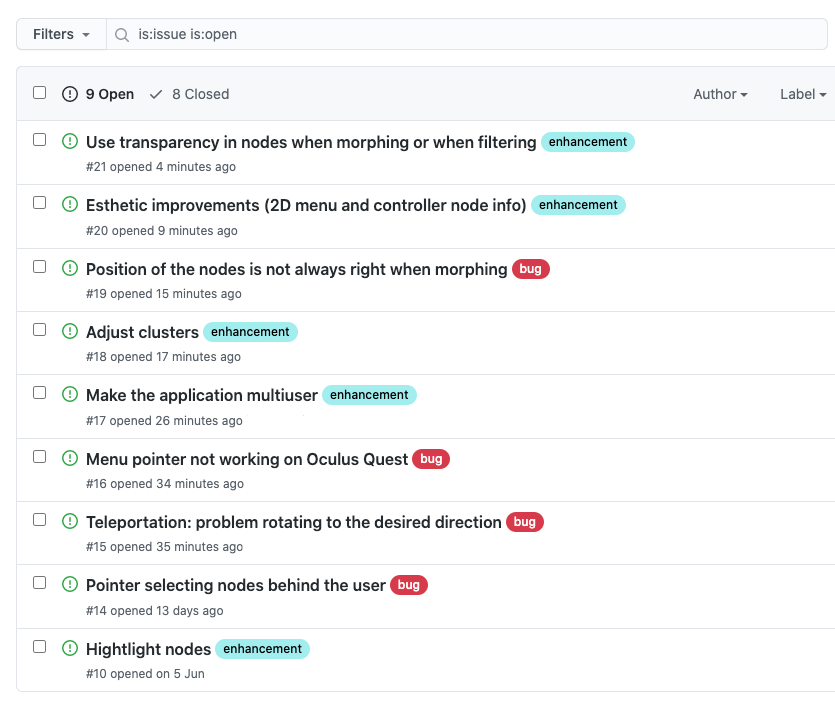
\includegraphics[width=\textwidth]{issues_github}
    \caption{List of issues from Github. They are tagged with "bug" or "enhancement" to specify what kind of issue it is about.}
    \label{fig:issues}
\end{figure}
